\chapter{Organización}
\section{Introducción}
Como se menciona en la primera parte el proyecto el objetivo del trabajo es presentar una arquitectura que mejore la sinergia en su actual plataforma web, para poder entender como se mejora la sinergia es necesario definir cual es la estructura de la organización y con que parte de la organización interactua la actual plataforma web. En este capitulo se hablara principalmente de la estructura que es la organización su misión, vision, objetivos y una vista a su estructura con elementos como elorganigrama, las funciones del negocio, el proceso y los servicios ofrecidos.
\newpage
\section{Nombre de la Organización}
La organización es llamada IEEE Sección Colombia ya que es una unidad organizacional dentro de la estrucutra de la organización del IEEE (Institute of Electrical and Electronics Engineers)

Siendo parte de la estructura organizacional del IEEE hereda su misión, visión y objetivos
\section{Misión}
 El proposito central del IEEE es fometar el desarrollo de la tecnologia y la excelencia en benefició de la humanidad.\cite{IEEEMisionVision}
\section{Visión}
IEEE será esencial para la comunidad técnica mundial y para los profesionales técnicos de todo el mundo, y será universalmente reconocido por las contribuciones de la tecnología y de los profesionales técnicos en la mejora de las condiciones globales.
\section{Objetivos Organizacionales}
\begin{itemize}
	\item  Expanda y permitir comunidades dinámicas, ágiles, flexibles y diversas para ayudar a personas de todo el mundo a compartir, colaborar, establecer redes, debatir y relacionarse entre sí.
	\item Proporcionar foros técnicamente vitales para la discusión, desarrollo y la diseminación de conocimiento autorizado relacionado con las tecnologías tradicionales, al mismo tiempo que concentramos más nuestros recursos en servir a los profesionales que trabajan en tecnologías emergentes y disruptivas.
	\item Dirige los esfuerzos humanitarios en todo el mundo para utilizar la tecnología para resolver los problemas más desafiantes del mundo.
	\item Aproveche la información relacionada con la tecnología de IEEE para proporcionar a los gobiernos, ONG y otras organizaciones y al público con recomendaciones innovadoras y prácticas para abordar los problemas de política pública.
\end{itemize}
\newpage
\section{Organigrama}

\begin{figure}[ht]
	\centering
	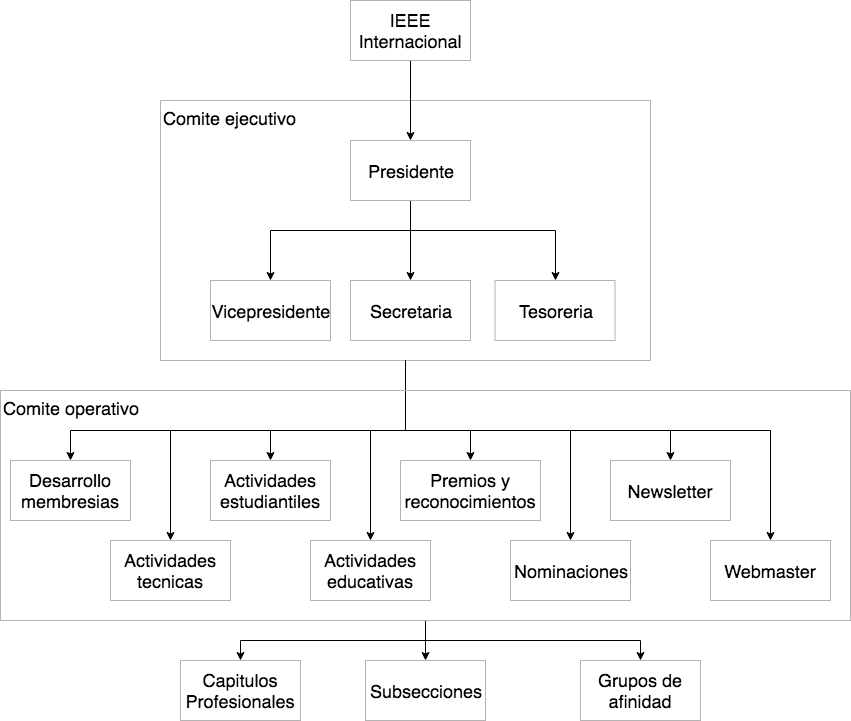
\includegraphics[width=1.2\linewidth]{arquitectura_diseno/imgs/organigrama}
	\caption{Organigrama de IEEE Sección Colombia}
	\label{fig:organigrama}
\end{figure}

\newpage
\section{Funciones del Negocio}
\begin{itemize}
	\item Postularce como organizadores de eventos internacionales del IEEE para que se hagan en Colombia
	\item Postular eventos que se quieran hacer en Colombia para que hagan parte de los eventos apoyados por el instituto
	\item Generar reportes anuales de los eventos organizados
	\item Generar documento de propuesta de eventos para organizar al año
	\item Apoyar a estudiante y profesionales interesados en la membresia y sus beneficios
	\item Disponer y ayudar a administrar los recursos ofrecidos por el instituto la las unidades organizaciones a su cargo (Capitulos, subsecciones y grupos de afinidad)
	\item Administrar, gestionar y ejecutar recursos destinados a las actividades orgaizadas por el comite operativo que complan con los objetivos del instituto.
\end{itemize}
\newpage
\section{Procesos del negocio}
El proceso de negoció varia deacuerdo a los servicios ofrecidos por la organización. En este caso se va a describir el proceso de negocio entorno a la organización de un congreso, siendo este servició con el que màs se destaca las sección.

\subsubsection{Estudio de factibilidad}
El primer paso para organizar un evento es evaluar el interes de los investigadores de la región en el tema, se evalua el lugar donde se puede hacer y un estimado en costos.

\subsubsection{Postulación}
Encaso de que el evento sea un evento que se organiza a nivel internacional se genera una postuación con el resultado del estudio para que un comite internacionar lo evalue y lo apruebe. encaso de ser un evento local se postula a un comite internacional para que lo avale como evento IEEE. Al final se definen las fechas del evento. 

\subsubsection{Selección del comite}
En esta etapa se define el staff del evento (presidente, tesorero, comite de evaluación, publication chair y web master) y se empiezan a asignar tareas.

\subsubsection{Construcción del call of papers}
En esta parte el comite de evaluación, el chair y el publicatión chair definen los temas con los que deben ir relacionados los papers que se van a resivir para evaluar. al final el web master debe publicarlo y encargarse de sudifución.

\subsubsection{Resepción y evaluación de articulos}
Se resiven los articulos de los investigadores interesados en participar en el evento. Estos luego son evaluados por el comite evaluador y se seleccionan los mejores trabajos. 

\subsubsection{Inscripción}
Se habilita la plataforma para que los autores aprovados puedan inscribirse al congreso

\subsubsection{Busqueda de Conferensistas}
El comite apoyado de la organización busca conferencisatas distiguidos que hablen sobre temás de interes entorno a la tematica del evento.

\subsubsection{Registro}
El dia uno del evento se registran a todos los participantes, generalmente este registro incluye un kit con memorias del evento.

\subsubsection{Conferencias y ponencias}
Con un comite generalmente de estudiantes voluntarios se gestiona la logistica del evento, verifican que los ponentes de los papers y los conferencistas puedan presentar su trabajo.

\subsubsection{Cierre}
El cierre incluye la entrega de certificados a todos los participantes incluyento al comite, voluntarios y conferencistas y la publicación de los trabajos expuestos en las bases de datos de IEEE

\newpage
\section{Servicios}
\begin{itemize}
	\item Organizar congresos con call of papers para promover la investigación den diferentes areas de tecnologia
	\item Organizar actividades de difución de la tecnologia como conferencias y talleres
	\item Apoyar a los mimbros de la organización con dudas sobre benefición y opciones que ofrece la membresia
	\item Apoyar a organizaciones como ONGs y universidades en el desarrollo de actividades que promuevan la visión de la organización.
\end{itemize}
\newpage
\section{Productos}
Basicamente hay 3 productos principales ofrecidos por IEEE Sección colombia.
\begin{itemize}
	\item Organización de congresos que promuevan la investiación en areas de la ingenieria
	\item Apoyar proyectos de indole humanitario que tengan que ver con tecnologia
	\item Brindar apoyo a los miembros con temas relacionados con beneficios de la membresia.
\end{itemize}
\newpage